%%%%%%%%%%%%%%%%%%%%%%%%%%%%%%%%%%%%%%%%%%%%%%%%%%%%%%%%
%%%%%%%%%%%%%%%%%%%%%%%%%%%%%%%%%%%%%%%%%%%%%%%%%%%%%%%%
\section{Survival Analysis}
\label{additional:Survival}

Survival analysis is a subfield of statistics which examines problems involving the timing of events
such as death, component failure, or exiting a line of therapy after an adverse effect, in a population of subjects under study.
Using the appropriate models, quantities such as the lifetime, or failure rate, of a subject
can be estimated, as well as their dependence on other independent variables.
A variety of common models are available,
each with their own assumptions, capabilities, and limitations,
which make them best suited for certain applications.

%%%%%%%%%%%%%%%%%%%%%%%%%%%%%%%%%%%%%%%%%%%%%%%%%%%%%%%%
\subsection{Nomenclature}
\label{additional:Survival:Nomenclature}

\begin{symbollist}
	\item[Event] The event of interest in a study, \eg death, component failure\ldots
	\item[$t$] Time from the start of observation to an event, the conclusion of the study, or the withdrawal of a subject.
	\item[$T$] Time that an event occurred.
	\item[$x$] Independent variable(s) under consideration.
	\item[Censoring] Right\footnote{Left censored subjects enter the study after the event of interest has already occurred at an unknown $t < 0$.} censored subjects have no events during the observation period, either due to early withdrawal or the conclusion of the study. The true lifetime of these subjects is unavailable for analysis, \ie they have been censored.
	\item[$S\left(t\right)$] The survival function $S\left(t\right)$ is the probability that a subject survives longer than $t$, \ie $S\left(t\right) = P\left(T > t\right)$.
	\item[$F\left(t\right)$] The lifetime distribution function $F\left(t\right)$ is the complement of the survival function, \ie $F\left(t\right) = 1 - S\left(t\right) = P\left(T \leq t\right)$.
	\item[$f\left(t\right)$] The event density function $f\left(t\right)$ is the time derivative of the lifetime distribution function $F\left(t\right)$, $f\left(t\right) = \frac{dF}{dt} = -\frac{dS}{dt}$, if it exists.
	\item[$\lambda\left(t\right)$] The hazard function $\lambda\left(t\right)$ is the event rate at $t$ conditional on survival to time $t$, \ie $T > t$, see \cref{eq:Survival:hazard_def}. Any $\lambda\left(t\right)$ can be a hazard function, provided it satisfies \cref{eq:Survival:hazard_cond}.
	\item[$\Lambda\left(t\right)$] The cumulative hazard function $\Lambda\left(t\right)$ is the integral of $\lambda\left(t\right)$ with respect to time \cref{eq:Survival:cum_hazard:def}. Also see the relations in \cref{eq:Survival:cum_hazard:to_lambda,eq:Survival:cum_hazard:to_S}.
	\item[HR] The hazard ratio (HR) compares the hazards of two subsets of subjects partitioned by $x$ at time $t$, $\text{HR} = \lambda\left(x = 1\right) / \lambda\left(x=0\right)$. Also known as the relative risk.
\end{symbollist}

\begin{subequations}\label{eq:Survival:hazard_def}
\begin{align}
\lambda\left(t\right) dt &= P\left(T \leq t + dt \mid T > t\right),\,\text{as} \,\, dt \to 0 \label{eq:Survival:hazard_def:a} \\
\lambda\left(t\right) &= \lim_{dt \to 0} \frac{P\left(T \leq t + dt \cap T > t\right)}{P\left(T > t\right)\,dt} \label{eq:Survival:hazard_def:b} \\
&= \frac{1}{S\left(t\right)} \lim_{dt \to 0} \frac{P\left(t < T \leq t + dt\right)}{dt} \label{eq:Survival:hazard_def:c} \\
&= \frac{1}{S\left(t\right)} \lim_{dt \to 0} \frac{F\left(t + dt\right) - F\left(t\right)}{dt} \label{eq:Survival:hazard_def:d} \\
&= \frac{f\left(t\right)}{S\left(t\right)} = -\frac{1}{S} \frac{dS}{dt} \label{eq:Survival:hazard_def:e}
\end{align}
\end{subequations}

\begin{subequations}\label{eq:Survival:hazard_cond}
\begin{gather}
\forall t \geq 0, \, \lambda\left(t\right) \geq 0 \label{eq:Survival:hazard_cond:a} \\
\int_{0}^{\infty} \lambda\left(t\right) \, \dif t = \infty \label{eq:Survival:hazard_cond:b}
\end{gather}
\end{subequations}

\begin{subequations}\label{eq:Survival:cum_hazard}
\begin{gather}
\Lambda\left(t\right) = \int_{0}^{t} \lambda\left(u\right) \, \dif u = - \ln\left(S\left(t\right)\right) \label{eq:Survival:cum_hazard:def} \\
\lambda\left(t\right) = \frac{d\Lambda}{dt} = -\frac{1}{S} \frac{dS}{dt} \label{eq:Survival:cum_hazard:to_lambda} \\
S\left(t\right) = \exp\left(-\Lambda\left(t\right)\right) \label{eq:Survival:cum_hazard:to_S}
\end{gather}
\end{subequations}

%%%%%%%%%%%%%%%%%%%%%%%%%%%%%%%%%%%%%%%%%%%%%%%%%%%%%%%%
\subsection{Kaplan-Meier Model}
\label{additional:Survival:km}

The Kaplan-Meier model \cite{km} $\hat{S}_{\text{KM}}\left(t\right)$ is a non-parametric
estimate of $S\left(t\right)$ computed from empirical data.

\begin{equation}\label{eq:Survival:km}
\hat{S}_{\text{KM}}\left(t\right) = \prod_{i:\,t_{i} < t} \left(1 - \frac{d_{i}}{n_{i}}\right)
\end{equation}

\noindent Here the product is over all times $t_{i}$ at which $d_{i}$ events occurred,
and $n_{i}$ is the number of subjects still under study at $t_{i}$,
\ie subjects who have not had an event or been censured.
Due to its construction, $\hat{S}_{\text{KM}}\left(t\right)$ remains steady
between $t_{i}$ but drops vertically at each data point.
Therefore the derivative does not exist and we can not estimate $f\left(t\right)$ or $\lambda\left(t\right)$.
See \cref{fig:stanford_km:km} for one example of a Kaplan-Meier curve.

We can apply the Kaplan-Meier estimator to different subsets of subjects partitioned by a categorical variable $x$
in order to understand the dependence of $S\left(t\right)$ on $x$.
Note that $x$ can not be a continuous variable, and must be binned to integer classes if that is the case.

%%%%%%%%%%%%%%%%%%%%%%%%%%%%%%%%%%%%%%%%%%%%%%%%%%%%%%%%
\subsection{Exponential Model}
\label{additional:Survival:exp}

The exponential model is a parametric estimate of $S\left(t\right)$
valid when the hazard is expected to be constant with respect to $t$.
In nuclear physics\footnote{$\frac{dN}{dt} = -\lambda N$, $N\left(t\right) = N_{0} e^{-\lambda t}$,
half-life $t_{1/2} = \ln\left(2\right) / \lambda = \tau \ln\left(2\right)$, where $\tau$ is the time constant.} $\lambda\left(t\right) = \lambda$
decays per unit time really is a constant.
However, in most situations $\lambda = c$ is unrealistic over longer time scales,
as illustrated in \cref{additional:Survival:additional:bathtub}.
The exponential model can accommodate both categorical and continuous $x$ independent variables.

The survival function for the exponential model is simply

\begin{equation}\label{eq:Survival:exp}
\hat{S}_{\text{Exp}}\left(t\right) = e^{-\lambda t}
\end{equation}

\noindent where the hazard can be expanded in terms of $\mathbf{x}$, $\bm{\beta}$ as in a regression analysis:

\begin{equation}\label{eq:Survival:exp_lambda}
\begin{aligned}
\lambda\left(x\right) &= \exp\left(\beta_{0} + \sum_{j=1}^{n}\, \beta_{j} x_{j}\right) \\
\log\left(\lambda\right) &= \mathbf{x} \bm{\beta}
\end{aligned}
\end{equation}

\noindent Here we are making the {\em proportional hazards assumption},
\ie the differences in $\lambda$ between subgroups in $x_{j}$
are proportional\footnote{Really $\log\left(\lambda\right) \propto \beta$.} to $\beta_{j}$
and constant over $t$.
To find the best estimate of $\hat{\bm{\beta}}$,
$\lambda$ is used to derive a likelihood function which is
then optimized\footnote{The exact details of this optimization
are handled by common software libraries and are omitted here.
Similar approaches are also used to fit the later Weibull and Cox proportional-hazards models.}.

The hazard ratio for $x_{j}$ is:

\begin{equation}\label{eq:Survival:exp_HR}
\begin{aligned}
\text{HR}_{\text{Exp}} &= e^{\ldots+\beta_{j} 1+\ldots} / e^{\ldots+\beta_{j} 0+\ldots} \\
&= e^{\beta_{j}}
\end{aligned}
\end{equation}

\subsubsection{Weibull Model}
\label{additional:Survival:weibull}

The Weibull model expands on the standard exponential model
by introducing a shape parameter $k$ to adjust the time dependence of the hazard:

\begin{equation}\label{eq:Survival:weibull}
\begin{aligned}
\hat{S}_{\text{Weibull}}\left(t\right) &= e^{-\lambda_{\text{Weibull}} t} \\
\lambda_{\text{Weibull}} &= \exp\left(\beta_{0} t^{k} + \sum_{j=1}^{n}\, \beta_{j} x_{j}\right) \\
\text{HR}_{\text{Weibull}} &= e^{\beta_{j}}
\end{aligned}
\end{equation}

\noindent Here $\beta_{0}$ is the scale parameter of the hazard with respect to $t$,
while the other $\beta_{j}$ are scale parameters for the independent $x_{j}$.
For $k<0$ ($k>0$) the hazard monotonically decreases (increases) over time,
while $k=0$ returns the exponential model.
This allows phenomena such as burn in and compounding component failures to be modeled.
Numerous parameterizations and expansions of the Weibull model are available,
however they all share the property that
$\lambda = \exp\left(\beta_{0} f\left(t\right) + \sum_{j=1}^{n}\, \beta_{j} x_{j}\right)$
where $f\left(t\right)$ is a {\em known}, almost always monotonic, function of $t$.

%%%%%%%%%%%%%%%%%%%%%%%%%%%%%%%%%%%%%%%%%%%%%%%%%%%%%%%%
\subsection{Cox Proportional-Hazards Model}
\label{additional:Survival:cox}

The Cox proportional-hazards model \cite{cox} is a
semiparametric\footnote{Semiparametric as $\lambda_{0}\left(t\right)$ is unspecified, but $\bm{\beta}$ are still parameters of $\lambda$.} model
which further expands on the Weibull model by allowing
the time dependence of $\lambda$ to be an unknown function.
As the name suggests, the proportional hazards assumption is retained
allowing us to compute useful HR values
without even knowing $\lambda\left(t\right)$,
or $S\left(t\right)$\footnote{We can
plot Kaplan-Meier $S\left(t\right)$ curves of predictions from a Cox model,
after fitting the baseline hazard emperically on a reference subset,
but only at discrete values of $\mathbf{x}$.
See \cref{fig:cox:cox_age_baseline_survival} for one example.}.

In the Cox model we assume the hazard has the form of

\begin{equation}\label{eq:Survival:cox_lambda}
\lambda_{\text{Cox}} = \lambda_{0}\left(t\right) \exp\left(\sum_{j=1}^{n}\, \beta_{j} x_{j}\right)
\end{equation}

\noindent where $\lambda_{0}\left(t\right)$ is the baseline hazard, an unspecified function of $t$.
When computing hazard ratios $\lambda_{0}\left(t\right)$ then drops out:

\begin{equation}\label{eq:Survival:cox_HR}
\text{HR}_{\text{Cox}} = e^{\beta_{j}}
\end{equation}

%%%%%%%%%%%%%%%%%%%%%%%%%%%%%%%%%%%%%%%%%%%%%%%%%%%%%%%%
\subsection{Method Comparison}
\label{additional:Survival:comp}

\begin{table}[H]
\centering
\begin{tabular}{l|l|l}
\multicolumn{1}{c|}{Kaplan-Meier} & \multicolumn{1}{c|}{Exponential / Weibull} & \multicolumn{1}{c}{Cox} \\
\cline{1-3}
\begin{tabular}[c]{p{0.3\textwidth}}
Pro
\begin{itemize}
	\item Simple to compute and understand
	\item Can estimate $S$
\end{itemize}
\\
Con
\begin{itemize}
	\item No functional form
	\item Can \textbf{not} estimate HR
	\item Only can handle a few categorical $x$
\end{itemize}
\end{tabular}

&

\begin{tabular}[c]{p{0.3\textwidth}}
Pro
\begin{itemize}
	\item Can estimate $S$ and HR
\end{itemize}
\\
Con
\begin{itemize}
	\item $\lambda\left(t\right) = c$ can be unrealistic
	\item Weibull: $\lambda = f\left(t\right)$ of a known form
\end{itemize}
\end{tabular}

&

\begin{tabular}[c]{p{0.3\textwidth}}
Pro
\begin{itemize}
	\item $\lambda$ can be an unknown function of $t$
	\item Can estimate HR
\end{itemize}
\\
Con
\begin{itemize}
	\item Can \textbf{not} estimate $S$
\end{itemize}
\end{tabular}

\\
\end{tabular}
\end{table}

%%%%%%%%%%%%%%%%%%%%%%%%%%%%%%%%%%%%%%%%%%%%%%%%%%%%%%%%
\subsection{Model Assumptions}
\label{additional:Survival:assumptions}

\begin{enumerate}[noitemsep]
\item Any censoring is non-informative, \ie censoring is uncorrelated with the probabilities of different event outcomes.\label{item:Survival:assumptions:censoring}
\item Survival times $t$ are uncorrelated across subjects.\label{item:Survival:assumptions:t_uncorr}
\item $\mathbf{x}$ is constant over time, per subject.\label{item:Survival:assumptions:X_constant}
\item Hazards are proportional, \ie hazard ratios are constant over time.\label{item:Survival:assumptions:prop_hazard}
\item $\log\left(\lambda\right)$ is linear with respect to the continuous $x_{j}$ independent variables.\label{item:Survival:assumptions:X_linearity}
\end{enumerate}

\cref{item:Survival:assumptions:censoring,item:Survival:assumptions:t_uncorr,item:Survival:assumptions:X_constant}
are assumptions for all survival models, while
\cref{item:Survival:assumptions:prop_hazard,item:Survival:assumptions:X_linearity}
apply to the exponential, Weibull and Cox models.

\subsubsection{Tests and Corrections}
\label{additional:Survival:assumptions:tests_and_corrections}

\begin{itemize}[noitemsep]
\item[\cref{item:Survival:assumptions:censoring}.] Exploratory data analysis to detect differences in $\mathbf{x}$ distributions between censored and non-censored subjects. If violated, better input data is needed, redesign study.

\item[\cref{item:Survival:assumptions:t_uncorr}.] Exploratory data analysis, study design question. If violated, redesign study.

\item[\cref{item:Survival:assumptions:X_constant}.] Exploratory data analysis, study design question. If unavoidable, can try a more complex time dependent covariate model.

\item[\cref{item:Survival:assumptions:prop_hazard}.] Check with a Schoenfeld test or complementary log-log plot. If violated, stratify problematic $x_{j}$ variables into separate models, or use more complex models with time dependent $\beta$ coefficients.

\item[\cref{item:Survival:assumptions:X_linearity}.] Check the appropriate residual plots. If violated, try to linearize the offending continuous $x_{j}$ with a transformation or bin to a categorical variable.
\end{itemize}

\subsubsection{Schoenfeld Test}
\label{additional:Survival:assumptions:schoenfeld}

Schoenfeld residuals are similar in concept to normal residuals in regression analyses,
but instead of looking at the difference between the true and estimated values of $y$,
$\hat{\bm{\epsilon}} = \mathbf{y} - \mathbf{X} \hat{\bm{\beta}}$,
we look at the difference in $\bm{\beta}$ and $\hat{\bm{\beta}}$ for a particular $y$ value.
In this way, Schoenfeld residuals represent the difference in the
coefficient $\beta_{j}$ fit from all data points, and a single point.
To validate the proportional hazards assumption
the Schoenfeld residuals \cite{schoenfeld} must not change over time.
An example Schoenfeld residual plot is provided in
\cref{fig:cox:schoenfeld_residuals}.
Besides graphically looking at the residuals,
we can use $\chi^{2}$-tests to compute {\pvalue}s
to test the null hypothesis, \ie the Schoenfeld residuals and time are independent.
In this case, the proportional hazards assumption is supported
if we find large, non-significant {\pvalue}s.

\subsubsection{Complementary Log-Log Plot}
\label{additional:Survival:assumptions:cloglog}

For categorical variables we can look at the
complementary log-log plot
of $\log\left(-\log\left(S\left(t\right)\right)\right)$ versus $\log\left(t\right)$.
An example complementary log-log plot is provided in \cref{fig:stanford_cloglog}.
If the different categories have parallel curves
the proportional hazards assumption is
valid for the variable in question.

\subsubsection{Other Residual Plots}
\label{additional:Survival:assumptions:linearity}

To test the linearity of $\log\left(\lambda\right)$ with respect to the continuous $x_{j}$
we may plot the Martingale residuals.
Martingale residuals range from $-\infty$ to $1$
and measure the difference between the observed and predicted survival for a subject.
Subjects who have an event ``to early'' will have residuals near one,
where as subjects who have an event ``to late'' will have residuals near $-\infty$.
The mean of the residuals should be $0$, see \cref{fig:cox:martingale_residuals:prediction} for an example.
We can also plot the Martingale residuals versus any particular $x_{j}$
to judge the linearity along that specific dimension, see \cref{fig:cox:martingale_residuals:age}.

The Martingale residuals can be symmetrized into deviance residuals,
which have a mean of $0$ and standard deviation of $1$,
for easier interpretation, see \cref{fig:cox:outliers:deviance}.

Lastly, we can recompute the model fit leaving out event $i$
and measure the resulting change in the $\beta_{j}$ coefficients,
$\hat{\Delta}_{ij} = \hat{\beta}_{j} - \hat{\beta}_{j}^{\left(i\right)}$, \ie ``dfbeta''.
Plotting $\hat{\Delta}_{ij}$ versus event number $i$
can then point to overly influential events, see \cref{fig:cox:outliers:dfbeta}.

%%%%%%%%%%%%%%%%%%%%%%%%%%%%%%%%%%%%%%%%%%%%%%%%%%%%%%%%
\subsection{Additional Concepts}
\label{additional:Survival:additional}

\subsubsection{Logrank Test}
\label{additional:Survival:additional:logrank}

The logrank test is a method for comparing the survival functions of two different groups.
Survival status versus group membership $2\times2$ tables are computed at each distinct time $t_{i}$,
before being combined into one $\chi_{\text{logrank}}^{2}$ test statistic
with the Cochran-Mantel-Haenszel test\footnote{Sometimes
the logrank test is itself referred to as the Mantel-Haenszel test.}.
$\chi_{\text{logrank}}^{2}$ approximately has the $\chi^{2}$ distribution with 1 degree of freedom,
allowing the production of {\pvalue}s to test the null hypothesis
that there is {\em no} difference in the group's survival functions.

The logrank test is most accurate when the proportional hazards assumption is satisfied,
but is still somewhat usable if the difference in hazard ratios has only one sign,
\ie the $S\left(t\right)$ curves do not cross as can be checked with a complementary log-log plot.
In \R the logrank test can be computed with the \texttt{survdiff} function,
with the parameter $\rho$ left at its default value of $0$.

\subsubsection{Concordance Statistic}
\label{additional:Survival:additional:concordance}

The concordance statistic, or C-statistic, is a measure of goodness of fit
for binary problems such as survival analysis or logistic regression.
Two subjects are picked at random, if the ordering of model's predicted $\hat{y}$ values
agrees with the order of the observed $y$ values, the pair of subjects is said to be concordant.
In terms of survival analysis, if the subject of the pair the model predicted to have a longer lifetime
in fact did have the longer observed lifetime, the pair is concordant.

By measuring the fraction of concordant pairs over all pairs,
we arrive at the concordance statistic which ranges from $0$ to $1$,
with $0.5$ being equivalent to random guessing and $1$ representing ideal performance.
The ROC AUC and C-statistic are equivalent in
logistic regression\footnote{The pairs here must have a $y=0$ and $y=1$ subject, with the $y=1$ subject receiving the higher $\hat{y}$.}.

\subsubsection{Odds, Log Odds, and the Odds Ratio in Relation to the Hazard Ratio}
\label{additional:Survival:additional:odds}

To begin, note that the odds of an event occurring are:

\begin{equation}\label{eq:Survival:odds}
\text{Odds} = \frac{P\left(\text{Occurring}\right)}{P\left(\text{Not Occurring}\right)} = \frac{p}{1-p}
\end{equation}

\noindent For example, when rolling a fair dice, $\text{odds}\left(3\right) = (1/6) / (5/6) = 0.2$, or 1:5.
Odds may vary from $0$ to $\infty$, with $1$ representing fair odds.
As such, they are not symmetric and are somewhat unwieldy.
For this reason it is common to take the log of the odds,
\ie log odds, which varies symmetrically between $-\infty$ and $\infty$, with 0 being fair.

An odds ratio is simply the ratio of two odds.
If we take a biased coin with $\text{odds}\left(\text{heads}\right) = 2$, or 2:1 in favor of heads,
the odds ratio between the biased coin and a fair coin is $2/1 = 2$,
\ie the odds of getting heads with the biased coin are 2 times that of the fair coin.
If desired, we can similarly take the ratio of log odds.

In logistic regression models, see \cref{regression:logistic},
it is possible to compute an odds ratio for the input feature $x_{j}$,
representing the change in odds due to a one unit increase in $x_{j}$.
This is very similar in concept to the HR,
which itself is a ratio of two probabilities from different sets of subjects separated by $x_{j}$.
However, as odds and probability are different quantities,
relative risks, including the HR, are not equivalent to odds ratios.
In some cases the relative risk and odds ratio may have similar values,
see Table 3 of \cite{pmid26623395},
but it is important to remember they are ultimately different concepts.

\subsubsection{Expected Future Lifetime}
\label{additional:Survival::additional:efl}

The expected future lifetime $\expval{T-t_{0}}$ is the
expected additional time of survival for a subject having already survived to $t_{0}$.
We can derive $\expval{T-t_{0}}$ \cref{eq:Survival:efl_der:efl}
from the probability of an event occurring between $t_{0}$ and $t_{0} + t$ \cref{eq:Survival:efl_der:P}
using the prior work of \cref{eq:Survival:hazard_def} and integration by parts:

\begin{subequations}\label{eq:Survival:efl_der}
\begin{gather}
P\left(T \leq t_{0} + t \mid T > t_{0}\right)
= \frac{F\left(t_{0} + t\right) - F\left(t_{0}\right)}{S\left(t_{0}\right)} \label{eq:Survival:efl_der:P} \\
\text{PDF}
= \frac{d}{dt} P\left(T \leq t_{0} + t \mid T > t_{0}\right)
= \frac{f\left(t_{0} + t\right)}{S\left(t_{0}\right)} \label{eq:Survival:efl_der:pdf} \\
\expval{T-t_{0}}
= \int_{0}^{\infty} t \, \text{PDF} \, \dif t
= \frac{1}{S\left(t_{0}\right)} \int_{0}^{\infty} S\left(t\right) \, \dif t \label{eq:Survival:efl_der:efl}
\end{gather}
\end{subequations}

\subsubsection{Bathtub Curve}
\label{additional:Survival:additional:bathtub}

In reliability engineering the hazard function of many components
can be estimated as a three part ``bathtub'' curve.
Initially the failure, \ie event, rate decreases as defective components fail early,
before reaching a constant plateau where failures are essentially random events.
As components wear out and reach the end of their useful lifetimes, the failure rate increases again.
Combining these three effects produces a bathtub-shaped curve, as seen in \cref{fig:bathtub_curve}.
We can model these situations with the Cox proportional-hazards model,
or a Weibull model with an appropriately shaped $\lambda\left(t\right)$.

\begin{figure}[H]
\centering
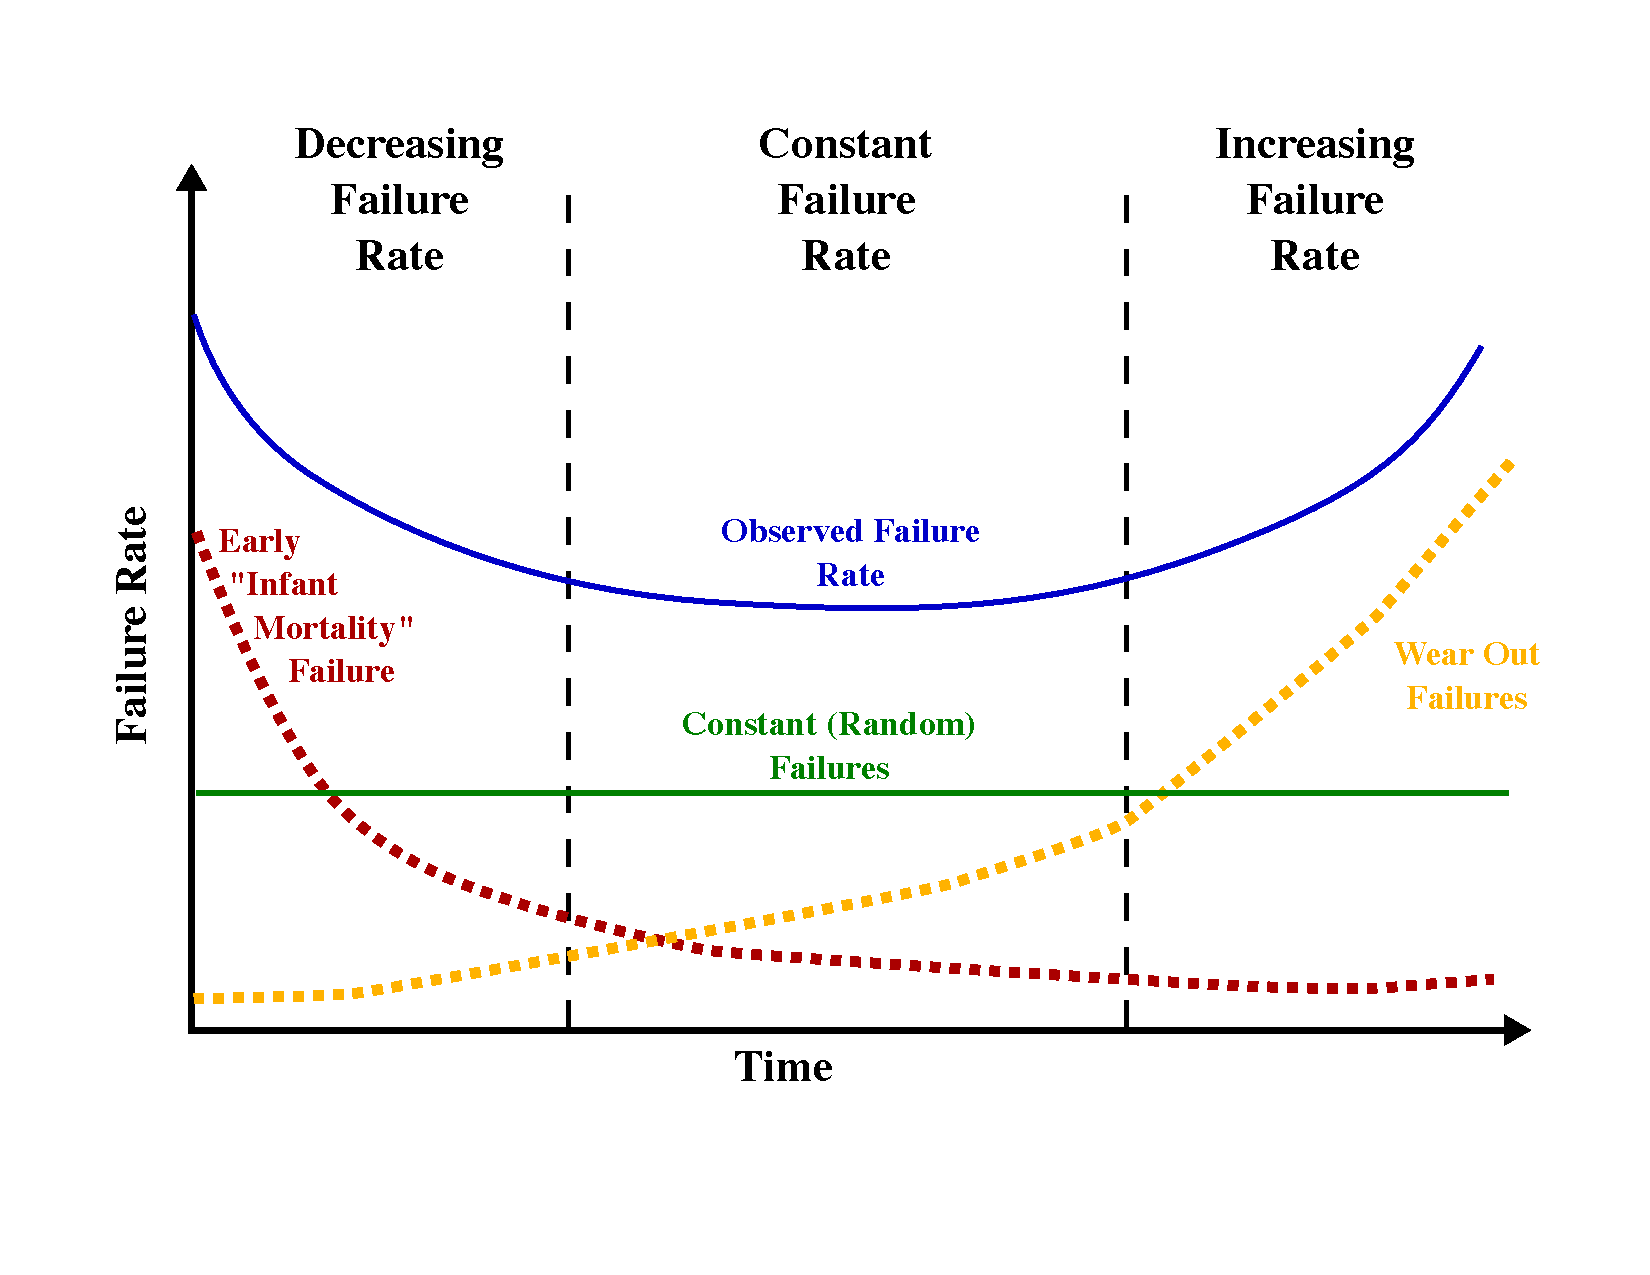
\includegraphics[width=0.7\textwidth]{figures/survival/bathtub_curve}
\vspace{0.2cm}
\caption{
Illustration of a bathtub curve hazard function, by \href{https://en.wikipedia.org/wiki/File:Bathtub_curve.svg}{Wyatts}.
}
\label{fig:bathtub_curve}
\end{figure}

%%%%%%%%%%%%%%%%%%%%%%%%%%%%%%%%%%%%%%%%%%%%%%%%%%%%%%%%
\subsection{Example \R Code}
\label{additional:Survival:Rcode}

A simple example survival analysis in \R utilizing the built-in
\texttt{stanford2} Stanford heart transplant dataset is provided in this section.
The examples here have been adapted from Mike Marin's
\href{https://www.youtube.com/playlist?list=PLqzoL9-eJTNDdnKvep_YHIwk2AMqHhuJ0}{series of lectures},
and \href{http://www.sthda.com/english/wiki/cox-model-assumptions}{notes} available from the STHDA.
The full \R code can also be found in
\href{https://github.com/mepland/data_science_notes/blob/main/sections/appendixes/additional/example_survival.R}{\texttt{example\_survival.R}}.
An equivalent analysis has also been performed in \python using the
\href{https://lifelines.readthedocs.io/en/latest}{\texttt{lifelines}} package,
see
\href{https://github.com/mepland/data_science_notes/blob/main/sections/appendixes/additional/example_survival.ipynb}{\texttt{example\_survival.ipynb}}.

The status variable represents the event, death of a patient, as $\text{status}=1$,
and the censoring of a patient as $\text{status}=0$.
Three independent variables $x$ are available,
age in years,
age categories - under or over 40,
and the numeric T5 mismatch score between donor and recipient.

\begin{figure}[H]
\centering
  \begin{subfigure}[c]{0.48\textwidth}\centering
  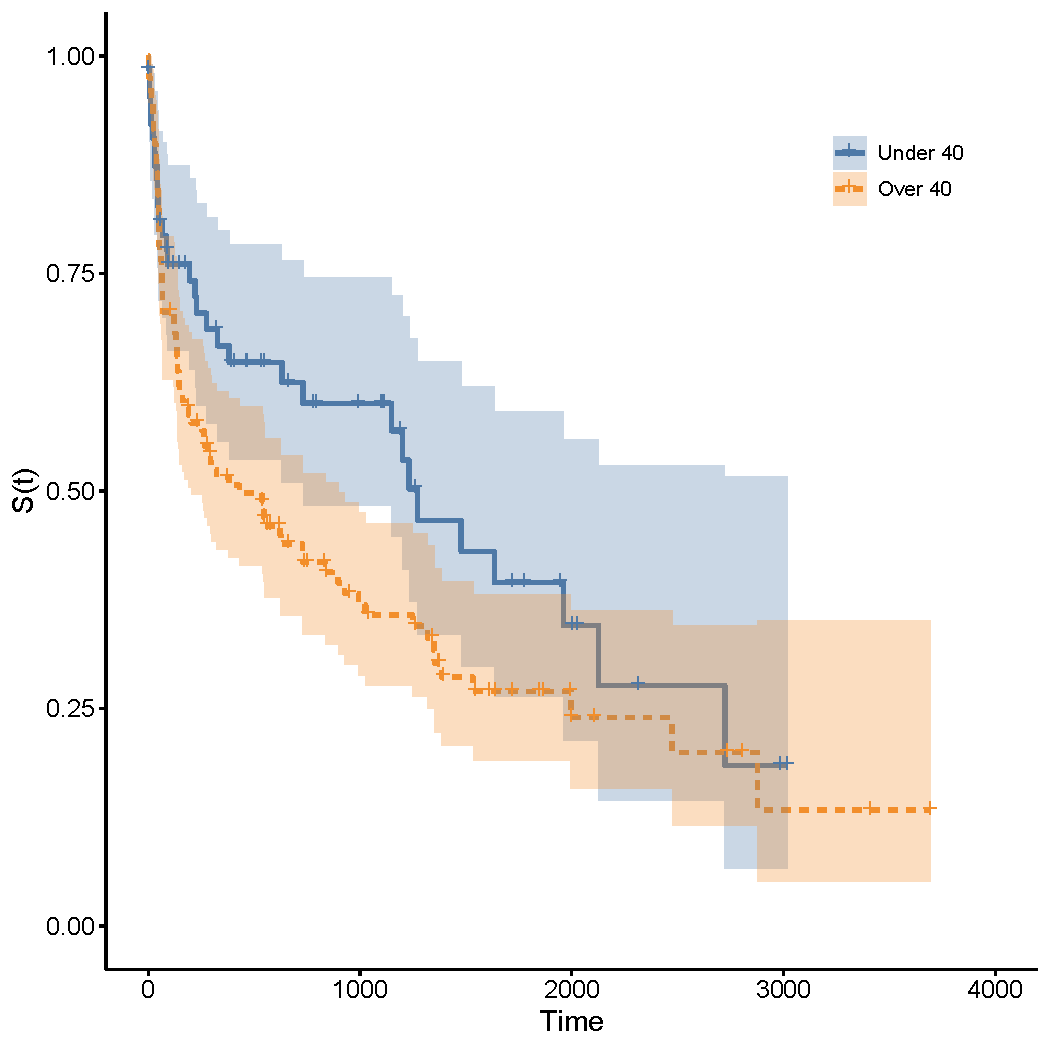
\includegraphics[width=\textwidth]{figures/survival/stanford_km}
  \caption{Kaplan-Meier}
  \label{fig:stanford_km:km}
  \end{subfigure}
  ~
  \begin{subfigure}[c]{0.48\textwidth}\centering
  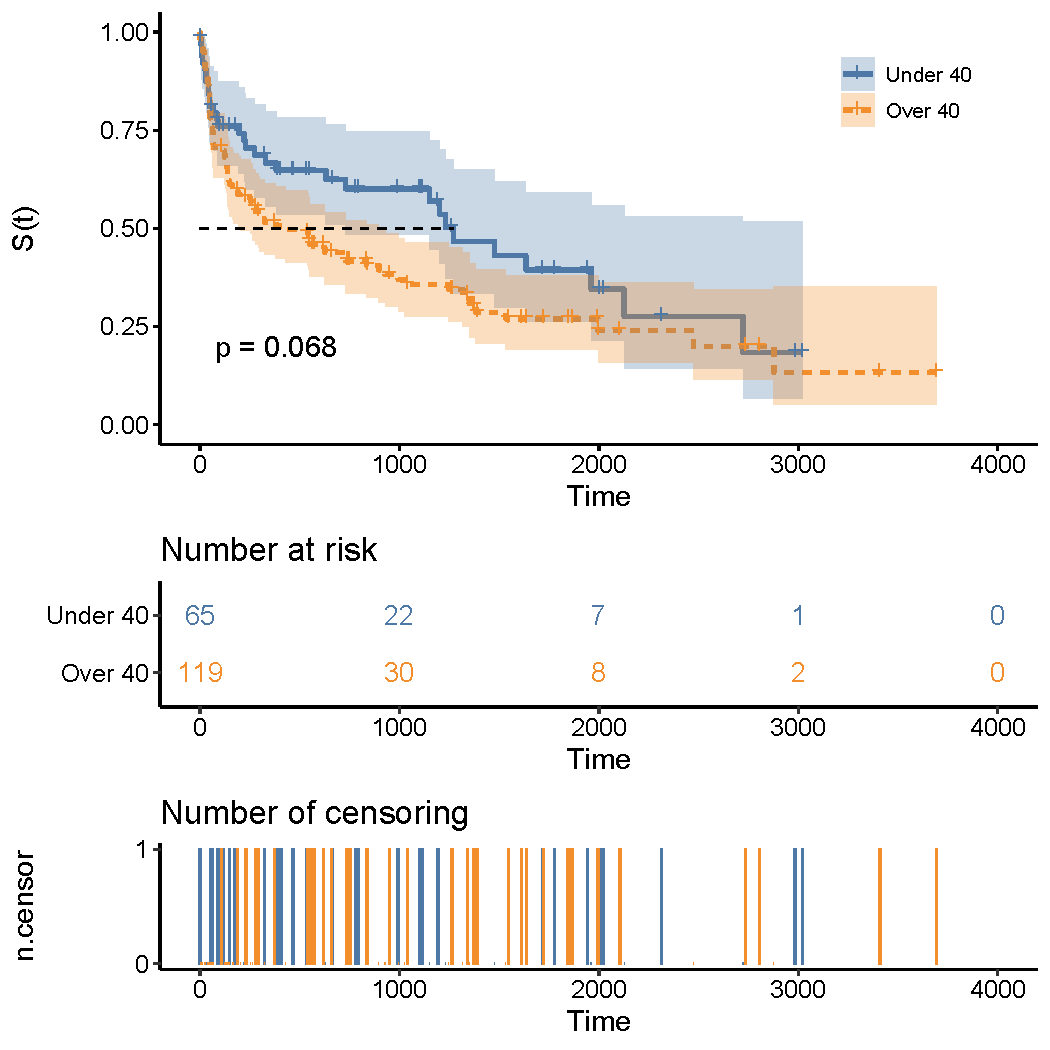
\includegraphics[width=\textwidth]{figures/survival/stanford_km_annotated}
  \caption{Annotated}
  \label{fig:stanford_km:annotated}
  \end{subfigure}
\caption{
Kaplan-Meier plot of the Stanford heart transplant dataset. Censored patients are displayed with marks.
The version on the right adds additional annotations, such as
subplots for patients at risk and censoring events,
the \pvalue from the logrank test, and a median reference line.
}
\label{fig:stanford_km}
\end{figure}

\subsubsection{Initialization}
\label{additional:Survival:Rcode:init}

Here we load the necessary packages and data,
and create the categorical age variable \texttt{agecat}.

\begin{lstlisting}[language=R]
> install.packages(c("survival", "survminer"))
> library("survival")
> library("survminer")

> df <- stanford2
> df$agecat <- cut(df$age, breaks=c(0,40, Inf), labels=c('Under 40', 'Over 40'), right=FALSE)
> df <- df[with(df, order(time)),]

> df[1:5,c('time', 'status', 'age', 'agecat', 't5')]
    time status age   agecat   t5
21   0.5      1  41  Over 40 0.87
133  1.0      1  21 Under 40 0.47
184  1.0      0  27 Under 40   NA
16   1.0      1  54  Over 40 0.47
183  2.0      0  39 Under 40   NA
> summary(df[c('time', 'age', 'agecat', 't5')])
      time              age             agecat          t5
 Min.   :   0.50   Min.   :12.00   Under 40: 65   Min.   :0.000
 1st Qu.:  64.75   1st Qu.:35.00   Over 40 :119   1st Qu.:0.690
 Median : 351.00   Median :44.00                  Median :1.040
 Mean   : 696.94   Mean   :41.09                  Mean   :1.117
 3rd Qu.:1160.75   3rd Qu.:49.00                  3rd Qu.:1.460
 Max.   :3695.00   Max.   :64.00                  Max.   :3.050
                                                  NA's   :27
\end{lstlisting}

\subsubsection{Kaplan-Meier Model}
\label{additional:Survival:Rcode:km}

The Kaplan-Meier model for this data partitioned by \texttt{agecat}
shows a median survival time of \num{1271} (\num{431}) for patients Under 40 (Over 40).
The logrank test, \texttt{survdiff}, returned a \pvalue of \num{0.07},
thus while the survival curves appear visually different we {\em can not} reject the null hypothesis,
the survival curves are the same, at the standard \pvalue of \num{0.05}.

\begin{lstlisting}[language=R]
> km.model <- survfit(Surv(time, status) ~ agecat, data=df, type='kaplan-meier')
> summary(km.model)$table
                records n.max n.start events   *rmean *se(rmean) median 0.95LCL 0.95UCL
agecat=Under 40      65    65      65     32 1520.783   220.1031   1271     731      NA
agecat=Over 40      119   119     119     81 1123.229   143.3516    431     202     897

> survdiff(Surv(time, status) ~ agecat, data=df)
Call:
survdiff(formula = Surv(time, status) ~ agecat, data = df)

                  N Observed Expected (O-E)^2/E (O-E)^2/V
agecat=Under 40  65       32     41.3      2.10      3.32
agecat=Over 40  119       81     71.7      1.21      3.32

 Chisq= 3.3  on 1 degrees of freedom, p= 0.07

> pdf('~/stanford_km.pdf')
> ggsurvplot(km.model, xlab='Time', ylab='S(t)', size = 1, linetype = 'strata', palette=c('#4e79a7', '#f28e2b'), conf.int = TRUE, legend = c(0.85, 0.85), legend.y = 1, legend.title = '', legend.labs = c('Under 40', 'Over 40'))
> dev.off()

> pdf('~/stanford_km_annotated.pdf')
> ggsurvplot(km.model, xlab='Time', ylab='S(t)', size = 1, linetype = 'strata', palette=c('#4e79a7', '#f28e2b'), conf.int = TRUE, legend = c(0.85, 0.85), legend.y = 1, legend.title = '', legend.labs = c('Under 40', 'Over 40'),
pval = TRUE, # Add survdiff p-value
risk.table = TRUE, # Absolute number at risk
risk.table.y.text.col = FALSE, risk.table.col = "strata",
ncensor.plot = TRUE, # plot censored patients vs time
surv.median.line = "h", # add horizontal median
)
> dev.off()
\end{lstlisting}

\subsubsection{Cox Proportional-Hazards Model}
\label{additional:Survival:Rcode:cox}

Two Cox proportional-hazards models are demonstrated here,
the first using age alone and the second adding the T5 score.
To compare apples-to-apples, subjects with null T5 values are excluded from both models.

In the age alone model, the coefficient for age is
$\beta_{\text{age}} = \num{0.02990}$, giving a HR of
$\exp\left(\beta_{\text{age}}\right) = \num{1.03035}$.
The \SI{95}{\percent} confidence interval for the HR is {1.008} to \num{1.054}.
The \pvalue for $\beta_{\text{age}}$ is \num{0.00846},
thus we can reject the null hypothesis that $\beta_{\text{age}} = 0$.
We are also provided with three {\pvalue}s for the model as a whole;
\num{0.006} for the likelihood-ratio test,
\num{0.008} for the Wald test,
and \num{0.008} for the logrank test.
These test the null hypothesis that all $\beta_{i} = 0$.
Here all three tests reject the null hypothesis,
as could be expected since the single $\beta_{\text{age}}$ was significant,
but would be more interesting for higher dimensional models.
The concordance statistic of \num{0.595} is poor, but is better than random guessing.

In the extended mode the age HR is very similar, \num{1.03006},
while the T5 HR is \num{1.18579}.
We can interpret the second model's T5 HR as follows;
at a given instant in time, an individual of age $a$ is
\num{1.18579} times, \ie \SI{18.579}{\percent}, as likely to die as an individual of age $a+1$, when controlling for T5 score.
The inverse HR, $\exp\left(-\beta_{\text{age}}\right)$, where the reference group has been switched, is also provided for convenience.

We can compare the two nested models using a likelihood-ratio test.
The resulting large \pvalue of \num{0.3563} supports the null hypothesis,
thus we conclude there is not a statistically significant difference between the two models.
We can remove T5 from the model without a loss of predictive power in this case.

The baseline survival function for the age only model
is plotted in \cref{fig:cox:cox_age_baseline_survival}.
A more complete plot including a range of ages can be found in the
\href{https://github.com/mepland/data_science_notes/blob/main/sections/appendixes/additional/example_survival.ipynb}{\texttt{example\_survival.ipynb}} implementation.

\begin{lstlisting}[language=R]
> cox.model_age <- coxph(Surv(time, status) ~ age, data=df[!is.na(df$t5), ])
> summary(cox.model_age)
Call:
coxph(formula = Surv(time, status) ~ age, data = df[!is.na(df$t5),
    ])

  n= 157, number of events= 102

       coef exp(coef) se(coef)     z Pr(>|z|)
age 0.02990   1.03035  0.01136 2.633  0.00846 **
---
Signif. codes:  0 ‘***’ 0.001 ‘**’ 0.01 ‘*’ 0.05 ‘.’ 0.1 ‘ ’ 1

    exp(coef) exp(-coef) lower .95 upper .95
age      1.03     0.9705     1.008     1.054

Concordance= 0.595  (se = 0.034 )
Likelihood ratio test= 7.62  on 1 df,   p=0.006
Wald test            = 6.93  on 1 df,   p=0.008
Score (logrank) test = 7.01  on 1 df,   p=0.008

> pdf('~/stanford_cox_age_baseline_survival.pdf')
> ggsurvplot(survfit(cox.model_age, data=df[!is.na(df$t5), ]), xlab='Time', ylab='S(t)', size = 1, linetype = 'strata', palette=c('#4e79a7'), conf.int = TRUE, legend = c(0.85, 0.85), legend.y = 1, legend.title = '', legend.labs = c('Baseline Survival'))
> dev.off()

> cox.model_age_t5 <- coxph(Surv(time, status) ~ age + t5, data=df[!is.na(df$t5), ])
> summary(cox.model_age_t5)
Call:
coxph(formula = Surv(time, status) ~ age + t5, data = df[!is.na(df$t5),
    ])

  n= 157, number of events= 102

       coef exp(coef) se(coef)     z Pr(>|z|)
age 0.02961   1.03006  0.01136 2.608  0.00911 **
t5  0.17041   1.18579  0.18326 0.930  0.35243
---
Signif. codes:  0 ‘***’ 0.001 ‘**’ 0.01 ‘*’ 0.05 ‘.’ 0.1 ‘ ’ 1

    exp(coef) exp(-coef) lower .95 upper .95
age     1.030     0.9708     1.007     1.053
t5      1.186     0.8433     0.828     1.698

Concordance= 0.59  (se = 0.034 )
Likelihood ratio test= 8.47  on 2 df,   p=0.01
Wald test            = 7.81  on 2 df,   p=0.02
Score (logrank) test = 7.87  on 2 df,   p=0.02

> anova(cox.model_age, cox.model_age_t5, test='LRT')
Analysis of Deviance Table
 Cox model: response is  Surv(time, status)
 Model 1: ~ age
 Model 2: ~ age + t5
   loglik Chisq Df P(>|Chi|)
1 -447.29
2 -446.86 0.851  1    0.3563
\end{lstlisting}

\begin{figure}[H]
\centering
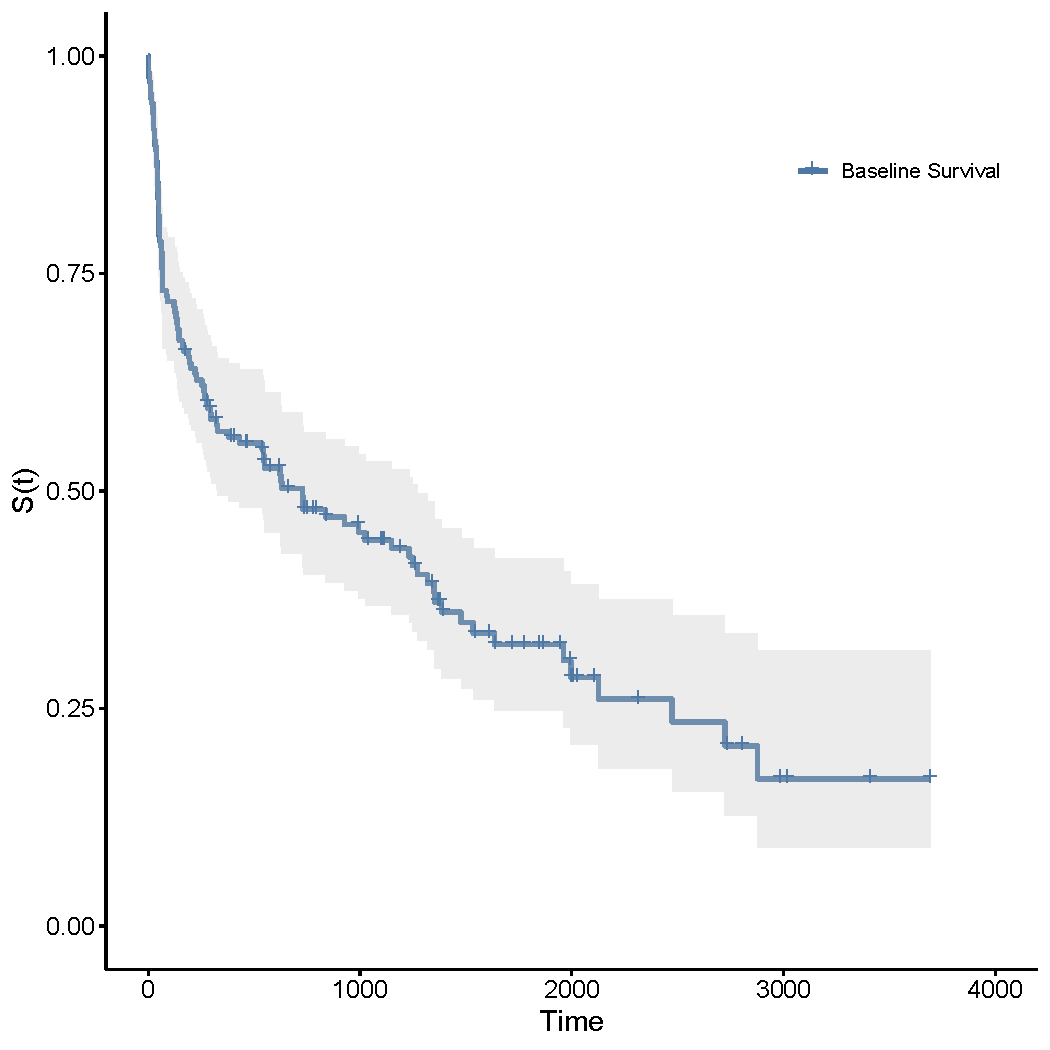
\includegraphics[width=0.7\textwidth]{figures/survival/stanford_cox_age_baseline_survival}
\vspace{0.2cm}
\caption{
Baseline survival function for
an univariate Cox model fit to the Stanford heart transplant dataset.
The documentation describing what reference value of age is utilized by \R here is unclear.
By comparing to the equivalent plot produced by \texttt{lifelines} in
\href{https://github.com/mepland/data_science_notes/blob/main/sections/appendixes/additional/example_survival.ipynb}{\texttt{example\_survival.ipynb}}
the age used appears to also be the mean.
}
\label{fig:cox:cox_age_baseline_survival}
\end{figure}

\subsubsection{Checking Assumptions}
\label{additional:Survival:Rcode:assumptions}

In this section we check the assumptions made by the Cox and Kaplan-Meier models.
The Schoenfeld test of the proportional hazards assumption
is implemented via the \texttt{cox.zph} function
for both example Cox models; age alone and age plus T5 score.
The large global {\pvalue}s, \num{0.38} and \num{0.25} respectively,
fail to reject the null hypothesis and show that the
proportional hazards assumption is valid here.
Additionally, we are provided with {\pvalue}s for each individual variable.

We can also check the proportional hazards assumption graphically
for categorical variables, see \cref{fig:stanford_cloglog}.
Note that the complementary log-log plot applies to the example Kaplan-Meier model,
while the rest of the plots apply to the age alone Cox model.
Please see the captions of
\cref{fig:cox:schoenfeld_residuals,fig:stanford_cloglog,fig:cox:martingale_residuals,fig:cox:outliers}
for further discussion of these diagnostic plots.

\begin{lstlisting}[language=R]
> cox.model_age.ph <- cox.zph(cox.model_age)
> cox.model_age.ph
       chisq df    p
age     0.76  1 0.38
GLOBAL  0.76  1 0.38

> cox.model_age_t5.ph <- cox.zph(cox.model_age_t5)
> cox.model_age_t5.ph
       chisq df    p
age     0.83  1 0.36
t5      2.06  1 0.15
GLOBAL  2.77  2 0.25

> pdf('~/stanford_cox_age_schoenfeld_residuals.pdf')
> ggcoxzph(cox.model_age.ph)
> dev.off()

> pdf('~/stanford_cloglog.pdf')
> plot(km.model, fun='cloglog', xlab='log(t)', ylab='log(-log(S(t)))', col=c('#4e79a7', '#f28e2b'))
> legend('bottomright', inset=.02, legend=c('Under 40', 'Over 40'), col=c('#4e79a7', '#f28e2b'), lty=1:2, box.lty=0)
> dev.off()

> pdf('~/stanford_cox_age_martingale_residuals.pdf')
> ggcoxdiagnostics(cox.model_age, type = "martingale", ox.scale='linear.predictions')
> dev.off()

> pdf('~/stanford_cox_age_martingale_residuals_age.pdf')
> ggcoxfunctional(Surv(time, status) ~ age, data = df)
> dev.off()

> pdf('~/stanford_cox_age_deviance_residuals.pdf')
> ggcoxdiagnostics(cox.model_age, type = "deviance", ox.scale='linear.predictions')
> dev.off()

> pdf('~/stanford_cox_age_dfbeta.pdf')
> ggcoxdiagnostics(cox.model_age, type = "dfbeta", ox.scale='observation.id')
> dev.off()

# export data for use in python with lifelines
write.csv(df[!is.na(df$t5), ],"~/stanford.csv", row.names = FALSE)
\end{lstlisting}

\begin{figure}[H]
\centering
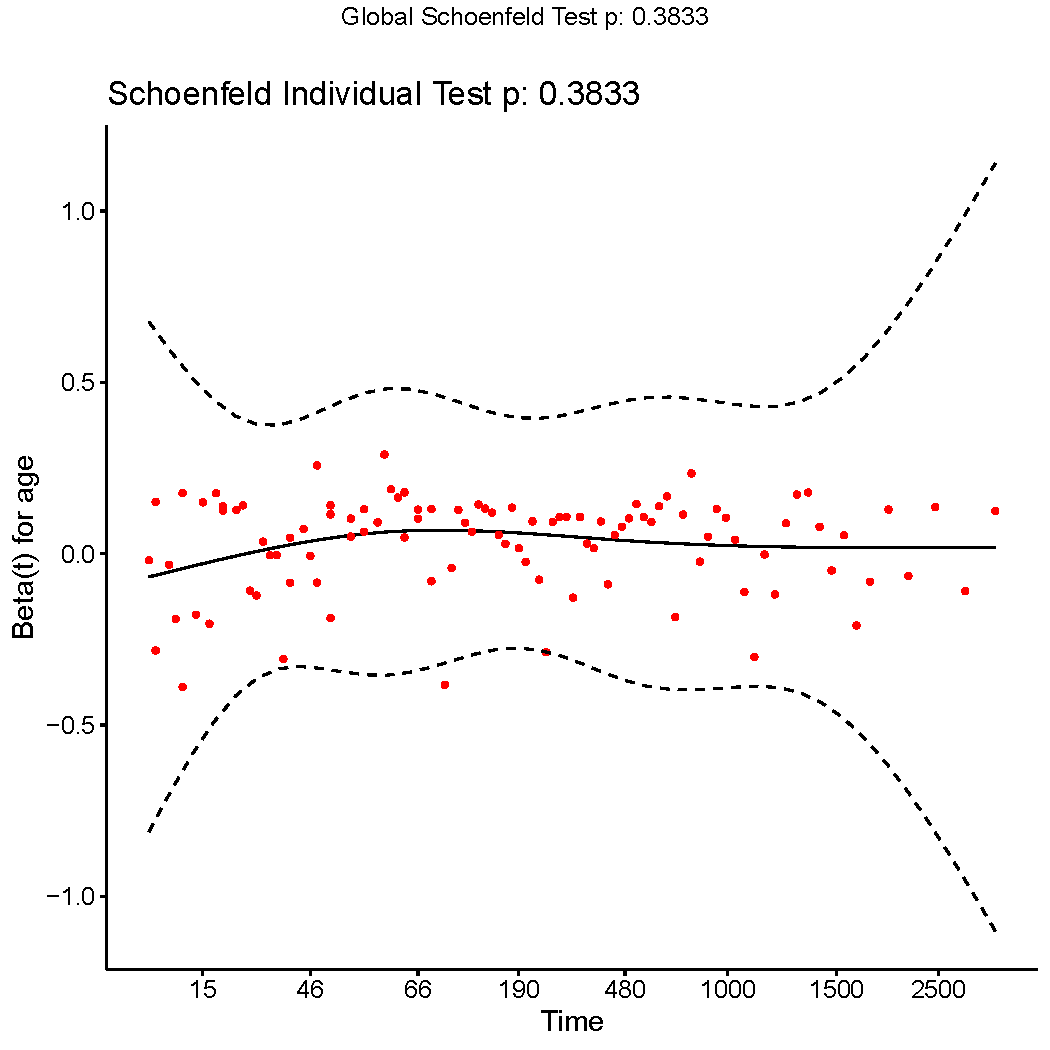
\includegraphics[width=0.7\textwidth]{figures/survival/stanford_cox_age_schoenfeld_residuals}
\vspace{0.2cm}
\caption{
Schoenfeld residual plot for
an univariate Cox model fit to the Stanford heart transplant dataset.
The residuals do not appear dependent on time,
which is supported by the non-significant \pvalue,
and shows that proportional hazards assumption
has been satisfied for this model.
Note that in a multivariate model we
would have a Schoenfeld residual plot for
each covariate.
}
\label{fig:cox:schoenfeld_residuals}
\end{figure}

\begin{figure}[H]
\centering
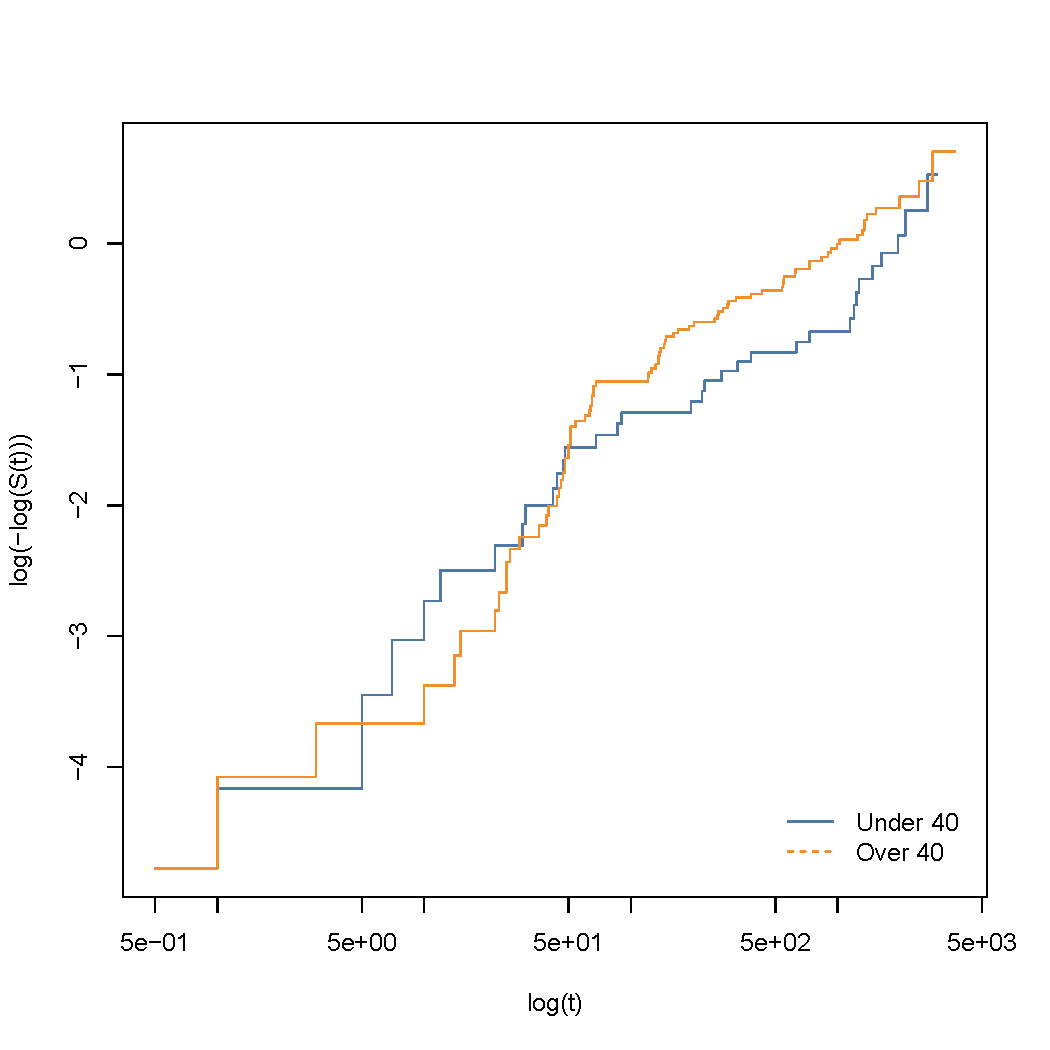
\includegraphics[width=0.7\textwidth]{figures/survival/stanford_cloglog}
\vspace{0.2cm}
\caption{
Complementary log-log plot for categorized patient age
in the Stanford heart transplant dataset.
These curves are not parallel,
the proportional hazards assumption is violated in this variable.
}
\label{fig:stanford_cloglog}
\end{figure}

\begin{figure}[H]
\centering
  \begin{subfigure}[c]{0.48\textwidth}\centering
  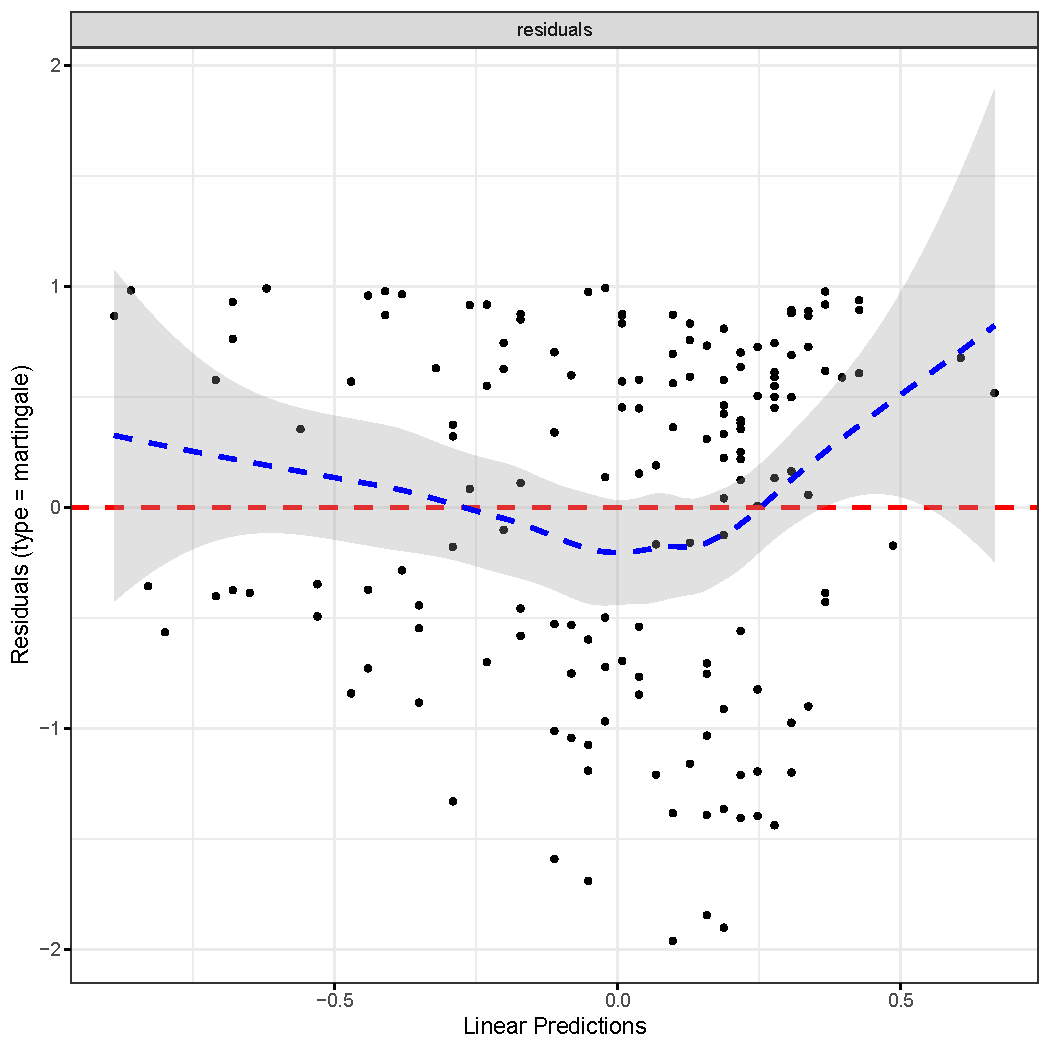
\includegraphics[width=\textwidth]{figures/survival/stanford_cox_age_martingale_residuals}
  \caption{vs Log Partial Hazard, \newline\ie Linear Predictions}
  \label{fig:cox:martingale_residuals:prediction}
  \end{subfigure}
  ~
  \begin{subfigure}[c]{0.48\textwidth}\centering
  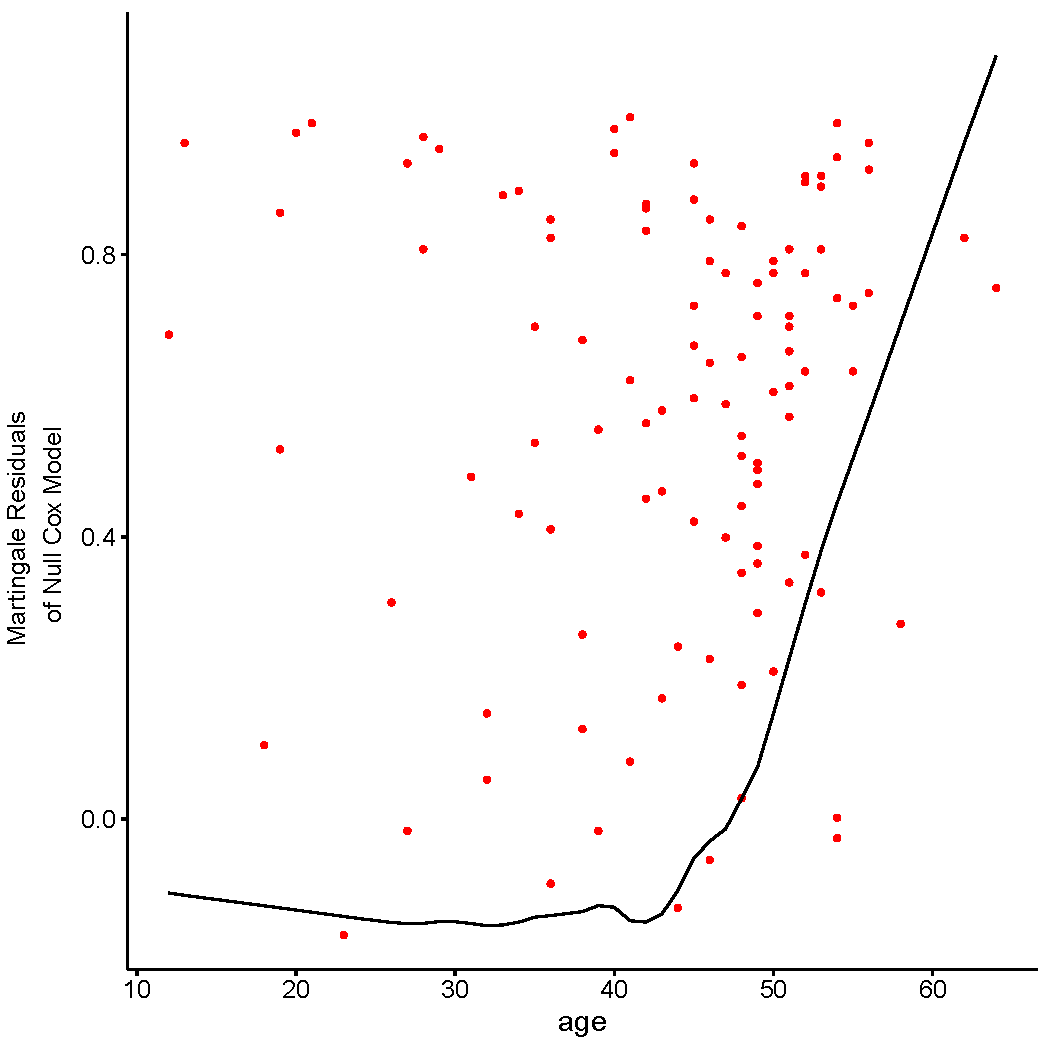
\includegraphics[width=\textwidth]{figures/survival/stanford_cox_age_martingale_residuals_age}
  \caption{vs Age}
  \label{fig:cox:martingale_residuals:age}
  \end{subfigure}
\caption{
Plots of Martingale residuals for
an univariate Cox model fit to the Stanford heart transplant dataset.
On the left, the residuals are plotted versus the
log of the partial hazard, \ie log hazard excluding the baseline hazard.
In \R this is known as \texttt{linear.predictors}, while in \texttt{lifelines} it is
\href{https://lifelines.readthedocs.io/en/latest/fitters/regression/CoxPHFitter.html\#lifelines.fitters.coxph_fitter.SemiParametricPHFitter.predict_log_partial_hazard}{log partial hazard}.
As can be seen in the blue fit, there is a slight nonlinearity.
On the right, residuals of the null model are plotted against the age variable alone.
For ages $\lesssim 40$, age appears to have a non-linear relationship with $\log\left(\lambda\right)$.
}
\label{fig:cox:martingale_residuals}
\end{figure}

\begin{figure}[H]
\centering
  \begin{subfigure}[c]{0.48\textwidth}\centering
  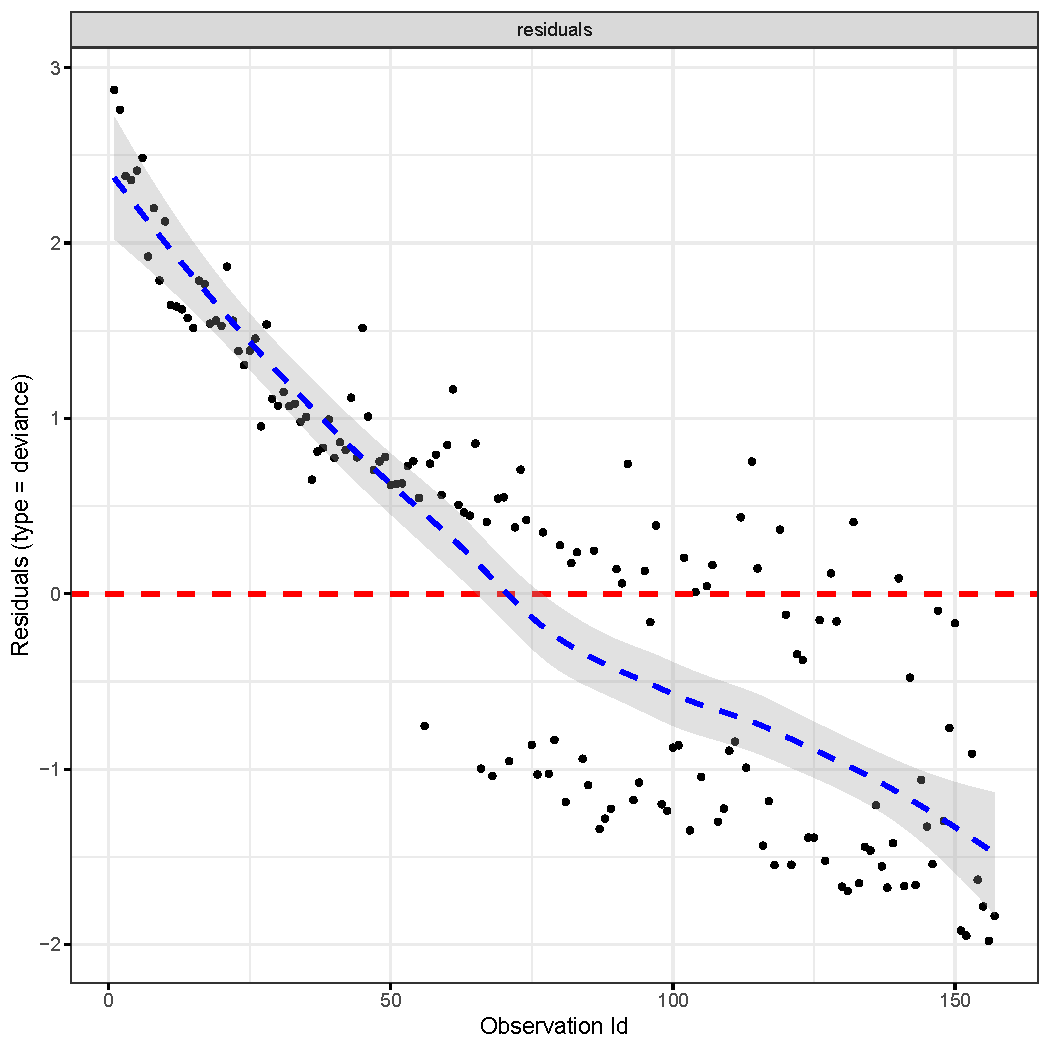
\includegraphics[width=\textwidth]{figures/survival/stanford_cox_age_deviance_residuals}
  \caption{Deviance}
  \label{fig:cox:outliers:deviance}
  \end{subfigure}
  ~
  \begin{subfigure}[c]{0.48\textwidth}\centering
  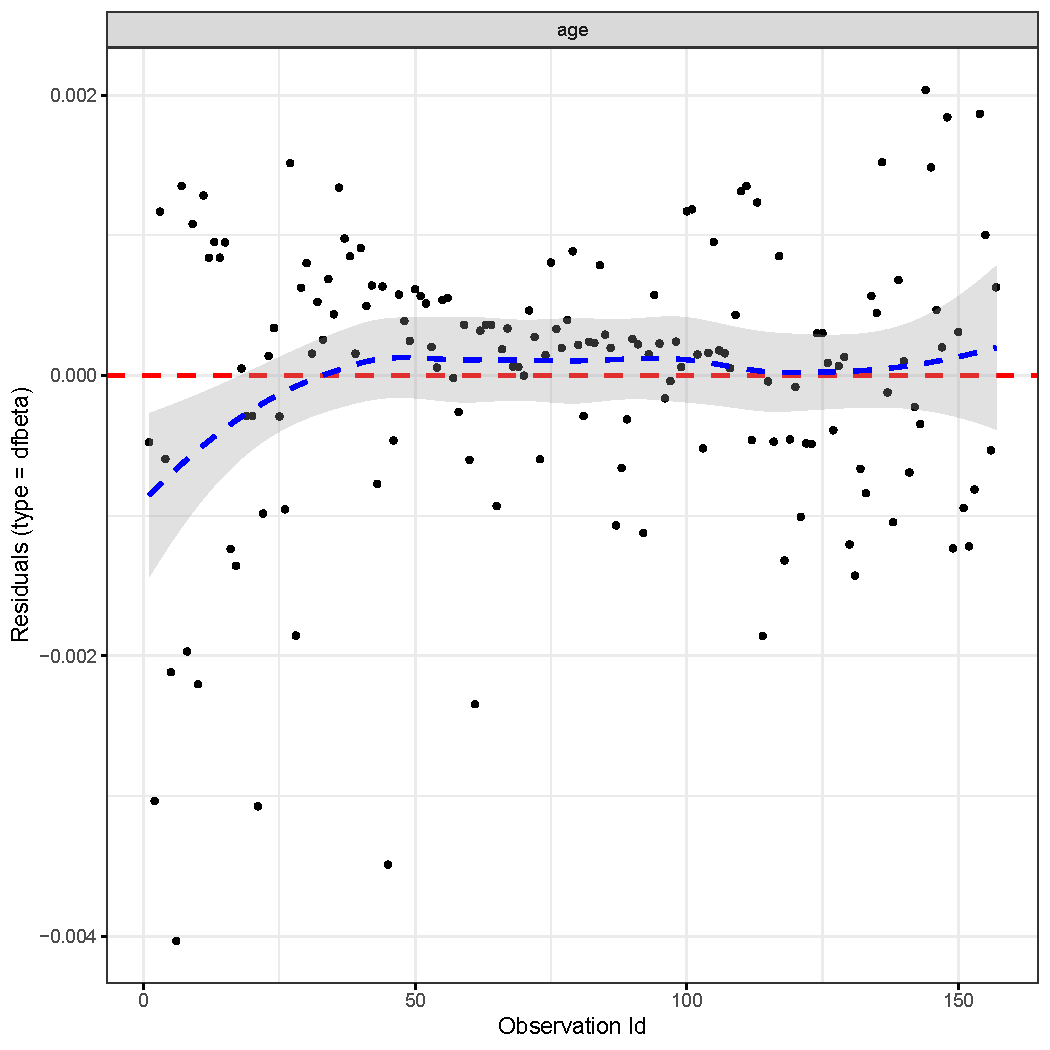
\includegraphics[width=\textwidth]{figures/survival/stanford_cox_age_dfbeta}
  \caption{dfbeta}
  \label{fig:cox:outliers:dfbeta}
  \end{subfigure}
\caption{
Additional residual plots for
an univariate Cox model fit to the Stanford heart transplant dataset.
On the left, the deviance residuals are plotted versus the
log of the partial hazard, \ie log hazard excluding the baseline hazard.
In \R this is known as \texttt{linear.predictors}, while in \texttt{lifelines} it is
\href{https://lifelines.readthedocs.io/en/latest/fitters/regression/CoxPHFitter.html\#lifelines.fitters.coxph_fitter.SemiParametricPHFitter.predict_log_partial_hazard}{log partial hazard}.
As can be seen in the blue fit, there is a slight nonlinearity.
On the right, the $\hat{\Delta}_{ij}$, \ie ``dfbeta'', residuals for age
are plotted against event number.
No event is particularly influential as $\abs{\hat{\Delta}_{ij}} \leq \num{0.004}$
for $\hat{\beta}_{\text{age}} = \num{0.02990}$.
}
\label{fig:cox:outliers}
\end{figure}
